\documentclass[multi=tikzpicture,border=7pt]{standalone}
\usepackage{ctex,amsmath,bm}
\usepackage{tikz}
\usetikzlibrary{arrows.meta,calc,angles,quotes,decorations.pathmorphing,patterns,positioning}
\tikzset{axis/.style={->,>=Stealth,thick},force/.style={->,>=Stealth,very thick},
flow/.style={->,>=Stealth,thick,blue!70!black},dim/.style={<->,>=Stealth,thin},
body/.style={draw=black,fill=blue!9,thick},point/.style={circle,fill=black,inner sep=1.6pt}}
\begin{document}

% 01 question-01
\begin{tikzpicture}[x=.9cm,y=.9cm]
  \filldraw[fill=blue!12,thick] (0,0) circle(1.55);
  \draw[thick,dashed] (0,0) circle(3.65);
  \fill (0,0) circle(2pt) node[below]{$O$};
  \filldraw[fill=orange!25,thick] (3.65,0) circle(.2) node[right]{$M$};
  \draw[dim] (0,.25)--(1.55,.25) node[midway,above]{$R$};
  \draw[dim] (0,-.3)--(3.65,-.3) node[midway,below]{$\alpha R$};
  \draw[flow] (3.65,.25)--(3.65,1.45) node[right]{$v_c$};
  \draw[force,red!75!black] (3.4,0)--(2.2,0) node[midway,below]{$u$};
  \node[align=center] at (0,-4.25){探测器在半径 $\alpha R$ 的圆轨道上\\仪器沿径向向内抛出};
\end{tikzpicture}

% 02 solution-01
\begin{tikzpicture}[x=1.1cm,y=1.1cm]
\filldraw[fill=blue!10](0,0)circle(1);\draw[dashed](0,0)circle(1.5);
\draw[red!75!black,very thick,domain=-180:180,samples=200]plot({1.5*cos(\x)/(1+.5*sin(\x))},{1.5*sin(\x)/(1+.5*sin(\x))});
\fill(0,0)circle(1.5pt)node[below left]{$O$};\fill(1.5,0)circle(2pt)node[below right]{$S$};\fill(0,1)circle(2pt)node[above left]{近地点 $R$};
\draw[force,red!75!black](1.5,0)--(.7,0)node[midway,above]{$u_0$};\draw[force,blue!70!black](1.5,0)--(2.3,0)node[midway,above]{$w$};\draw[flow](1.5,0)--(1.5,1.1)node[right]{$v_c$};
\draw[dim](0,-.35)--(1.5,-.35)node[midway,below]{$\alpha R$};
\node[align=center]at(0,-3.7){示例 $\alpha=1.5$，$e_i=0.5$\\$r=\alpha R/[1+(\alpha-1)\sin\varphi]$\\抛出点有径向速度，不是拱点};
\end{tikzpicture}

% 03 question-02
\begin{tikzpicture}[x=1cm,y=1cm]
  \draw[very thick] (-.8,0)--(9,0);
  \filldraw[fill=blue!15,thick] (1,.35) rectangle (2.4,1.15);
  \filldraw[fill=orange!18,thick] (6.7,.35) rectangle (8.1,1.15);
  \node at (1.7,.75){$A,m$}; \node at (7.4,.75){$B,m$};
  \draw[force] (1.1,1.55)--(3.1,1.55) node[midway,above]{$F$};
  \draw[dim] (2.4,-.45)--(6.7,-.45) node[midway,below]{$l$};
  \node at (4.2,-1.05){水平粗糙面，摩擦因数 $\mu$};
\end{tikzpicture}

% 04 solution-02
\begin{tikzpicture}[x=1cm,y=1cm]
\draw[axis](-.2,0)--(5,0)node[right]{$t$};\draw[axis](0,-.2)--(0,4.1)node[above]{$v$};
\draw[blue!70!black,very thick](0,0)--(1,2)--(1,0)--(2.333333,2.666667)--(2.333333,.666667)--(3.666667,3.333333)--(3.666667,1.333333)--(4.8,3.6);
\draw[green!55!black,thick](0,0)--(1,0)--(1,2)--(2.333333,.666667)--(2.333333,2.666667)--(3.666667,1.333333)--(3.666667,3.333333)--(4.8,2.2);
\node[blue!70!black]at(4.6,3.9){$v_A$};\node[green!55!black]at(4.6,1.9){$v_B$};\node at(2.3,-.8){$e=1,\alpha=3$：跳变交换速度};
\begin{scope}[shift={(7,1.5)}]
\draw[axis](-.2,0)--(4.5,0)node[right]{$g\tau/v_1$};\draw[axis](0,-1.3)--(0,2.3)node[above]{$v_A-v_B$};
\draw[blue!70!black,very thick](0,-1)--(2,1)--(2,-.5)--(3,.5)--(3,-.25)--(3.5,.25)--(3.5,-.125)--(3.75,.125)--(3.75,-.0625)--(3.875,.0625)--(4,0);
\draw[dashed](4,-1)--(4,1);\node[below]at(4,-1){$2$};
\node[align=center]at(2,-2.3){$e=1/2$：相对速度的真实锯齿\\累计时间 $2v_1/g$ 时共同速度仍为 $v_1/4$};
\end{scope}\end{tikzpicture}

% 05 question-03
\begin{tikzpicture}[x=.9cm,y=.9cm]
  \fill[gray!12] (-.5,-2.1) rectangle (8.4,2.1);
  \foreach \x/\y in {0/.8,.7/-1.2,1.6/1.4,2.5/-.3,3.4/1.1,4.2/-1.5,5.1/.3,6.0/1.5,7.0/-.8,7.8/.6}
    \fill[gray!65] (\x,\y) circle(1.8pt);
  \draw[fill=blue!12,thick,rounded corners] (-2.5,-.7) rectangle (-.6,.7);
  \draw[fill=orange!25,thick] (-2.9,-.35)--(-2.5,-.65)--(-2.5,.65)--(-2.9,.35)--cycle;
  \draw[force] (-2.8,1.15)--(-.65,1.15) node[midway,above]{$F_0$};
  \draw[dim] (-.5,-2.55)--(5.1,-2.55) node[midway,below]{$x$};
  \node at (3.8,2.55){静止星际尘埃：密度 $\rho_0$};
  \node at (-1.55,-1.2){飞船 $m_0,S$};
\end{tikzpicture}

% 06 solution-03
\begin{tikzpicture}[x=1cm,y=1cm]
\draw[axis](-.2,0)--(5.3,0)node[right]{$X$};\draw[axis](0,-.2)--(0,6.3)node[above]{$E/(m_0c^2)$};
\draw[blue!70!black,very thick](0,1)--(5,6);\node[left]at(0,1){$1$};\node at(2.8,4.8){$1+X$};
\begin{scope}[shift={(8,0)}]
\draw[axis](-.2,0)--(5.6,0)node[right]{$X$};\draw[axis](0,-.2)--(0,4.5)node[above]{$v/c$};
\draw[red!75!black,very thick,domain=0:5,samples=150]plot(\x,{4*sqrt(.5)*sqrt(\x*(\x+2))/(\x+1)});
\draw[dashed](0,2.828427)--(5.4,2.828427)node[right]{$1/\sqrt2$};\node[left]at(0,4){$1$};
\node[align=center]at(2.5,-.8){示例 $f=F_0/(F_0+\rho_0Sc^2)=1/2$\\$X=(F_0+\rho_0Sc^2)x/(m_0c^2)$};
\end{scope}\end{tikzpicture}

% 07 question-04
\begin{tikzpicture}[x=.9cm,y=.9cm]
  \begin{scope}
    \foreach \y in {-1.4,-.7,0,.7,1.4}{\draw[flow] (-3,\y)--(3,\y);}
    \draw[body,fill=gray!12] (0,0) circle(1.5);
    \node at (0,-2.1){(a) 匀强场中的孤立金属球};
    \node at (2.3,1.8){$\bm E_0$};
    \node[red!75!black] at (1.2,0){$+$}; \node[blue!70!black] at (-1.2,0){$-$};
  \end{scope}
  \begin{scope}[shift={(8.0,0)}]
    \draw[very thick] (-3,-1.5)--(3,-1.5);
    \foreach \x in {-2.4,-1.2,0,1.2,2.4}{\draw[flow] (\x,2.1)--(\x,-1.35);}
    \draw[body,fill=gray!12] (0,0) circle(1.5);
    \node at (0,-2.1){(b) 接地平面上的相切金属球};
    \node at (2.7,1.8){$\bm E_0$};
  \end{scope}
\end{tikzpicture}

% 08 solution-04
\begin{tikzpicture}[x=1cm,y=1cm]
\draw[very thick](-3.8,0)--(5.2,0)node[right]{接地平面 $z=0$};\draw[axis](-3.5,-4.2)--(-3.5,4.5)node[above]{$z$};
\draw[thick](0,2)circle(2);\draw[dashed](0,-2)circle(2);
\foreach \n/\yy in {1/3.15,2/2.35,3/1.55,4/.75}{
\fill[red!70!black](0,{2/\n})circle(2pt);\draw[thin](0,{2/\n})--(2.25,\yy);\node[right]at(2.25,\yy){$-q_0/\n^2$};
\fill[blue!70!black](0,{-2/\n})circle(2pt);}
\draw[force](.6,2.6)--(.6,1.6)node[right]{$\bm p_1$};\draw[force,blue!70!black](-2.8,3.5)--(-2.8,2.1)node[left]{$\bm E_0$};
\node[align=center]at(.5,-4.9){真实源 $z_n=R/n$，点电荷为负\\平面镜像电荷反号，轴向偶极矩同向};
\end{tikzpicture}

% 09 question-05
\begin{tikzpicture}[x=1cm,y=1cm]
\draw[fill=blue!7](-3,-1)rectangle(4,0);\node at(3.5,-.5){$n$};\node at(3,1.7){空气};\node at(3,-1.6){空气};
\draw[dashed](0,-1.4)--(0,2.5);
\draw[orange!80!black,very thick,->](-1.2,2.08)--(0,0);\draw[red!70!black,very thick,->](0,0)--(1.2,2.08)node[above]{上反射：$\pi$};
\draw[blue!70!black,thick,->](0,0)--(.4057,-1)--(.8114,0)--(2.0114,2.08)node[above]{下反射：$0$};
\draw[dim](-2.6,-1)--(-2.6,0)node[midway,left]{$d$};\node at(-.2,.8){$\alpha$};\node at(.8,-.65){$\varphi$};
\node at(.4,-2.2){两束反射光出射方向平行；液膜厚度放大示意};
\end{tikzpicture}

% 10 solution-05
\begin{tikzpicture}[x=1cm,y=1cm]
\draw[axis](0,0)--(8.1,0)node[right]{$\lambda$ (nm)};\draw[axis](0,-.2)--(0,4)node[above]{反射率（归一）};
\draw[blue!70!black,very thick,domain=380:700,samples=150]plot({(\x-380)/45},{3*sin(500/\x*90)^2});
\draw[red!70!black,very thick,domain=380:700,samples=150]plot({(\x-380)/45},{3*sin(539.5852967/\x*90)^2});
\draw[dashed](2.666667,0)--(2.666667,3);\draw[dashed](3.54634,0)--(3.54634,3);
\node[below]at(2.666667,0){$500$};\node[below]at(3.54634,-.5){$539.6$};\node[blue!70!black]at(1.3,3.7){斜入射};\node[red!70!black]at(5.5,3.7){正入射};
\node[align=center]at(3.8,-1.4){保持膜厚不变，增强峰向长波移动\\示意忽略折射率色散与振幅差异};
\end{tikzpicture}

% 11 question-06
\begin{tikzpicture}[scale=1.05]
  \foreach \i in {0,...,5}{\coordinate (P\i) at ({120-60*\i}:2.25);}
  \draw[thick] (P0)--(P1)--(P2)--(P3)--(P4)--(P5)--cycle;
  \foreach \i in {0,...,5}{\draw[thick] (0,0)--(P\i);}
  \fill (0,0) circle(2pt) node[below right]{$O$};
  \node[above] at (P0){$A$}; \node[below right] at (P3){$B$}; \node[left] at (P5){$C$};
  \node at (3.4,0){每边 $1\,\Omega$};
\end{tikzpicture}

% 12 solution-06
\begin{tikzpicture}[x=.85cm,y=.85cm]
  \begin{scope}
    \foreach \i in {0,...,5}{\coordinate (P\i) at ({120-60*\i}:2);}
    \draw[thick] (P0)--(P1)--(P2)--(P3)--(P4)--(P5)--cycle;
    \foreach \i in {0,...,5}{\draw[thick] (0,0)--(P\i);}
    \draw[force,purple!75!black] ($(P3)+(0,-1)$)--(P3) node[pos=.65,right]{$2\,\mathrm A$};
    \draw[force,purple!75!black] (P0)--++(0,1) node[above]{$2\,\mathrm A$};
    \node at (0,-2.8){分量一：$B\to A$};
  \end{scope}
  \begin{scope}[shift={(7,0)}]
    \foreach \i in {0,...,5}{\coordinate (Q\i) at ({120-60*\i}:2);}
    \draw[thick] (Q0)--(Q1)--(Q2)--(Q3)--(Q4)--(Q5)--cycle;
    \foreach \i in {0,...,5}{\draw[thick] (0,0)--(Q\i);}
    \draw[force,green!55!black] ($(Q0)+(0,1)$)--(Q0) node[pos=.15,right]{$3\,\mathrm A$};
    \draw[force,green!55!black] (Q5)--++(-1,0) node[left]{$3\,\mathrm A$};
    \node at (0,-2.8){分量二：$A\to C$};
  \end{scope}
\end{tikzpicture}

% 13 question-07
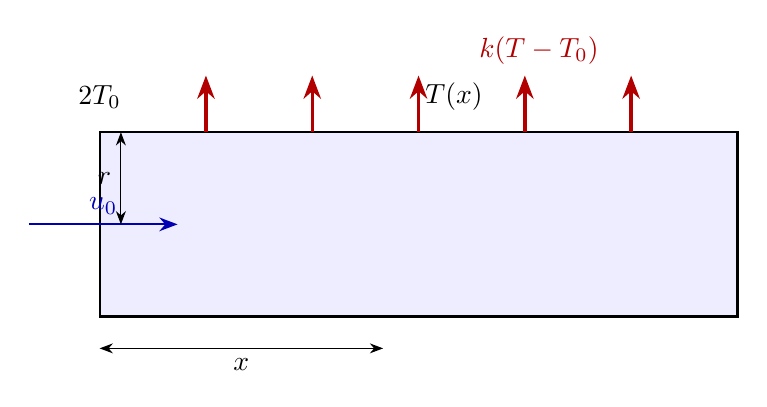
\begin{tikzpicture}[x=.9cm,y=.9cm]
  \draw[fill=blue!7,thick] (0,-1.3) rectangle (9,1.3);
  \draw[flow] (-1,0)--(1.1,0) node[midway,above]{$u_0$};
  \draw[dim] (.3,0)--(.3,1.3) node[midway,left]{$r$};
  \draw[dim] (0,-1.75)--(4,-1.75) node[midway,below]{$x$};
  \node at (0,1.8){$2T_0$}; \node at (5,1.8){$T(x)$};
  \foreach \x in {1.5,3,4.5,6,7.5}{\draw[force,red!70!black] (\x,1.3)--(\x,2.1);}
  \node[red!70!black] at (6.2,2.45){$k(T-T_0)$};
\end{tikzpicture}

% 14 solution-07
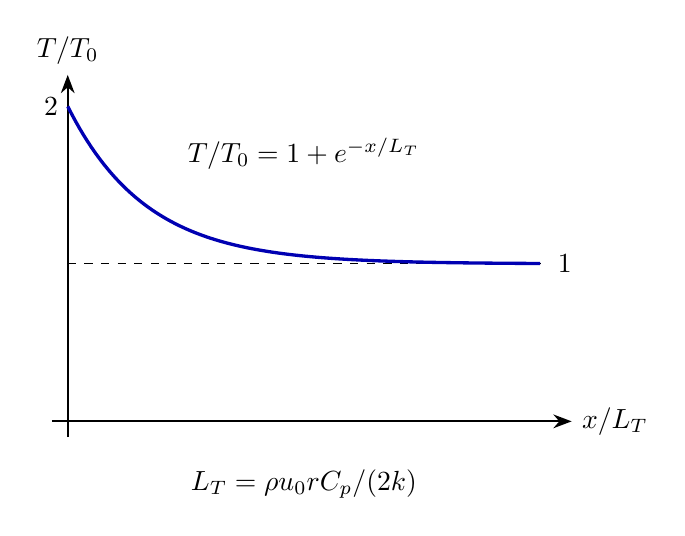
\begin{tikzpicture}
\draw[axis](-.2,0)--(6.4,0)node[right]{$x/L_T$};\draw[axis](0,-.2)--(0,4.4)node[above]{$T/T_0$};\draw[dashed](0,2)--(6.1,2)node[right]{$1$};\draw[blue!70!black,very thick,domain=0:6,samples=120]plot(\x,{2+2*exp(-\x)});\node[left]at(0,4){$2$};\node at(3,3.4){$T/T_0=1+e^{-x/L_T}$};\node at(3,-.8){$L_T=\rho u_0rC_p/(2k)$};\end{tikzpicture}

% 15 question-08
\begin{tikzpicture}[x=1cm,y=1cm]
\draw[axis](-.5,0)--(5.7,0)node[right]{$\rho$};\draw[axis](0,-.2)--(0,5.7)node[above]{$z$};\draw[fill=blue!8](-.2,0)rectangle(.2,5);
\foreach \h in {1,2,3,4}{\draw[blue!70!black,thick,domain=0:{2*sqrt(\h*(5-\h))},samples=100]plot({.2+\x},{\h-\x^2/(4*(5-\h))});\draw[flow](.2,\h)--(.7,\h);}
\draw[dim](-.7,0)--(-.7,5)node[midway,left]{$H$};\node at(2.5,-.8){各孔初始速度水平，射流立即下弯};
\end{tikzpicture}

% 16 solution-08
\begin{tikzpicture}[x=.9cm,y=.9cm]
\draw[axis](-.2,0)--(4.7,0)node[right]{$s/H$};\draw[axis](0,-.2)--(0,4.7)node[above]{$z/H$};
\fill[red!7](0,0)--(0,4)--(4,0)--cycle;\draw[red!70!black,thick](0,4)--(4,0);
\foreach \h in {.2,.4,.6,.8}{\draw[blue!70!black,thick,domain=0:{2*sqrt(\h*(1-\h))},samples=100]plot({4*\x},{4*(\h-\x^2/(4*(1-\h)))});}
\node[align=center]at(2,-.9){实际射流族与包络\\$z_{\max}/H=1-s/H$};
\begin{scope}[shift={(6.7,0)}]
\draw[axis](-.2,0)--(4.7,0)node[right]{$h/H$};\draw[axis](0,-.2)--(0,4.7)node[above]{$\rho/H$};
\draw[blue!70!black,very thick,domain=0:1,samples=150]plot({4*\x},{8*sqrt(max(0,\x*(1-\x)))});
\draw[dashed](2,0)--(2,4);\node[above]at(2,4){$1$};\node[below]at(2,0){$1/2$};
\node at(2,-.9){$\rho/H=2\sqrt{(h/H)(1-h/H)}$};
\end{scope}
\begin{scope}[shift={(13.4,0)}]
\draw[axis](-.2,0)--(4.7,0)node[right]{$\rho/H$};\draw[axis](0,-.2)--(0,4.7)node[above]{$h/H$};
\draw[red!70!black,very thick,domain=0:1,samples=150]plot({4*\x},{2+2*sqrt(max(0,1-\x^2))});
\draw[green!55!black,very thick,domain=0:1,samples=150]plot({4*\x},{2-2*sqrt(max(0,1-\x^2))});
\node[right]at(4,2){$1/2$};\node at(2,-.9){同一落点的高、低两支};
\end{scope}\end{tikzpicture}

\end{document}
